\subsection{WLAN - so funktioniert es}
\label{wlan}

\subsubsection{Auf dem Bot}
\label{wlan_auf_bot}
Als erstes muss das WLAN-Modul (WiPort) des ct-Bots konfiguriert werden.
Dazu verbintet man sich am besten mit diesem Modul über die serielle Schnitstelle.
(Ein spezieller USB-Adapter wird benötigt. Das rote Kabel muss rechts sein beim 
einstecken in den Roboter.) Um in das Konfigurationsmenü zu gelangen,
muss beim Start des Bots sofort x (mehrmals, um den Zeitpunkt nicht zu verpassen)
gedrück werden. Es erscheint folgende Ausgabe:
\begin{verbatim}
    MAC address 00204A96578C
    Software version V6.6.0.0 (080107) 
    Press Enter for Setup Mode
\end{verbatim}
Die Versionsnummer sollte übereinstimmen. Ältere Versionen haben andere
Konfigurationsmenüs. Nach dem betätigen der Enter-Taste wird der aktuelle
Konfigurationsstatus ausgegeben gefolgt von einem Menü.
Mit 7 können die Einstellungen zurückgesetzt werden.
Im Menüpunkt 0 (Server) sollte drauf geachtet werden das Wireless verwendet wird
und dem Bot die IP 192.168.0.Bot-Nummer zugeweisen wird.
Mit Menüpunkt 2 muss nun der Channel 2 eingestellt werden.
\begin{verbatim}
    Baudrate (9600) ? 57600
    I/F Mode (4C) ? 
    Flow (00) ? 
    Port No (10002) ? 
    ConnectMode (C0) ? CC
    Datagram Type (00) ? 01
    Send as Broadcast (N) ? 
    Remote IP Address : (000) 192.(000) 168.(000) 000.(000) 255
    Remote Port  (0) ? 10002
    Pack Cntrl  (00) ? 
    SendChar 1  (00) ? 
    SendChar 2  (00) ? 
\end{verbatim}

\noindent{Eine gültige Konfiguration könnte dann wie folgend aussehen:}
\begin{verbatim}
    *** basic parameters 
    Hardware: Ethernet TPI, WLAN 802.11bg
    Network mode: Wireless Only
    IP addr 192.168.0.9, no gateway set
    DNS Server not set

    *** Security
    SNMP is              enabled
    SNMP Community Name: public
    Telnet Setup is      enabled
    TFTP Download is     enabled
    Port 77FEh is        enabled
    Web Server is        enabled
    Web Setup is         enabled
    ECHO is              disabled
    Enhanced Password is disabled
    Port 77F0h is        enabled

    *** Channel 1
    Baudrate 9600, I/F Mode 4C, Flow 00
    Port 10001
    Connect Mode : C0
    Send '+++' in Modem Mode enabled
    Show IP addr after 'RING' enabled
    Auto increment source port disabled
    Remote IP Adr: --- none ---, Port 00000
    Disconn Mode : 00
    Flush   Mode : 00

    *** Channel 2
    Baudrate 57600, I/F Mode 4C, Flow 00
    Port 10002
    Connect Mode : CC
    Datagram Type 01
    Pack Cntrl:   00
    Remote IP Adr: 192.0.0.255, Port 10002


    *** Expert
    TCP Keepalive    : 45s
    ARP cache timeout: 600s
    CPU performance: Regular
    Monitor Mode @ bootup : enabled
    HTTP Port Number : 80
    SMTP Port Number : 25
    MTU Size: 1400
    Alternate MAC: disabled
    Ethernet connection type: auto-negotiate

    *** E-mail
    Mail server: 0.0.0.0
    Unit       : 
    Domain     : 
    Recipient 1: 
    Recipient 2: 

    - Trigger 1 
    Serial trigger input: disabled
      Channel: 1
      Match: 00,00
    Trigger input1: X
    Trigger input2: X
    Trigger input3: X
    Message : 
    Priority: L
    Min. notification interval: 1 s
    Re-notification interval  : 0 s

    - Trigger 2 
    Serial trigger input: disabled
      Channel: 1
      Match: 00,00
    Trigger input1: X
    Trigger input2: X
    Trigger input3: X
    Message : 
    Priority: L
    Min. notification interval: 1 s
    Re-notification interval  : 0 s

    - Trigger 3 
    Serial trigger input: disabled
      Channel: 1
      Match: 00,00
    Trigger input1: X
    Trigger input2: X
    Trigger input3: X
    Message : 
    Priority: L
    Min. notification interval: 1 s
    Re-notification interval  : 0 s

    *** WLAN 
    WLAN: enabled
    Topology: Ad-Hoc
    Network name: ctbot
    Country: US
    Channel: 11
    Security suite: none
    TX Data rate: 11 Mbps auto fallback
    Power management: not supported in adhoc mode
    Soft AP Roaming: N/A
\end{verbatim}


TODO:welche funktionen werden genutzt (Kevin: du hast rausgefunden wie das ganze zeug geht, kannst du das bitte beschreiben?\\
\subsubsection{Wlan Daten senden/empfangen}
\label{wlan_funktionen}


\textbf{Senden:} Das Schreiben/Senden von Daten ist relativ einfach da hierfür schon Funktionen zur Verfügung stehen die genau das für einen erledigen.\\
\\
\textbf{Empfangen:} Für das Empfangen gibt es die möglichkeit die in command.c definirte Funktion \verb|command_evaluate| zu erweitern. Das hat den Vorteil das jedes gültige Kommando das gelesen wird auch verarbeitet wird, solange dafür Code in \verb|command_evaluate| vorhanden ist.
Da wir aber nur unsere Kommandos verarbeiten mussten und zudem das Ziel hatten so wenig wie möglich in schon vorhandenen Dateien zu verändern, haben wir uns Hilfsfunktionen geschrieben.\\
\\
\verb|command_t* read_command()| liest ein Kommando in die schon vorhandene variable \verb|recived_command| in command.c ein und gibt einen Zeiger darauf zurück.\\
\\
Zum Lesen wird mit der schon vorhandenen Funktion \verb|uart_data_available| geschaut wieviel Bytes an Daten zum Lesen verfügbar sind.\\
\\
Wenn mindestens genug Daten für ein Kommando \verb|sizeof(command_t)| vorhanden sind, wird mit einer weiteren schon vorhandenen Funktion \verb|command_read| ein Kommando in die Puffervariable \verb|recived_command| eingelesen.\\
\\
Zuletzt wird mit der von uns zu command.c hinzugefügten Funktion \verb|get_recieved_command| ein Zeiger auf \verb|recived_command| zurückgegeben.\\
\\
\textbf{Payload Daten Auslesen:} Da nach einem Kommando noch zusätzlich Daten angehängt werden können, haben wir auch hierfür eine Funktion geschrieben.\\
\\
\verb|uint8_t* read_payload(command_t* cmd, uint8_t* buffer)| Liest die angehängten Daten des übergebenen Kommandos in den übergebenen buffer.\\ Hierfür wird auf die vorhandene Funktion \verb|low_read| zurückgegriffen.
\\


TODO: wie sieht die c-struktur aus (Andreas: schau nach, schreib auf!)\\

Damit der Bot ein WLAN-Paket als \textit{command} interpretiert, muss es einen Inhalt mit folgendem Aufbau besitzen:
\begin{figure}[H]
	\centering
	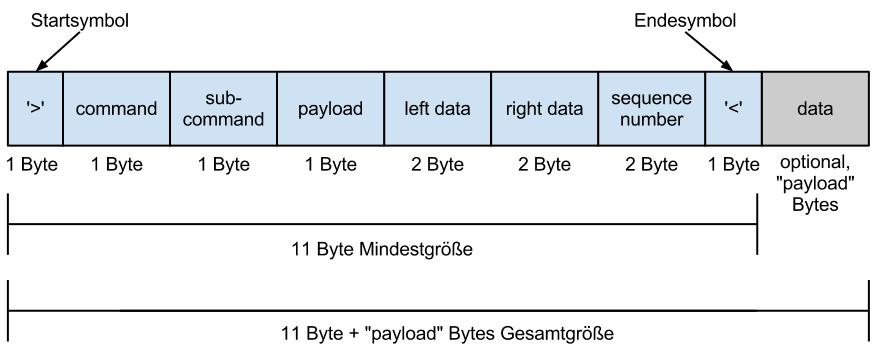
\includegraphics[scale=0.5]{pic/ctBotWlanAllgemein}
	\caption{Allgemeiner Aufbau eines \textit{commands} in einem WLAN-Paket}
	\label{ctBotWlanAllgemein}
\end{figure}


\subsubsection{Auf dem PC}
Um Daten an den Bot zu senden sind lediglich zwei Schritte erforderlich:
\begin{itemize}
	\item Zum WLAN verbinden\\
	Ist der Bot korrekt konfiguriert öffnet er ein Ad-Hoc-WLAN. Zu diesem muss man sich verbinden.
	\item Paket an den Bot senden bzw. Daten empfangen\\
	Ist man mit dem WLAN verbunden kann man einfach ein UDP-Paket mit einen speziellen Inhalt (siehe \ref{wlan_auf_bot}) an den Bot senden, so dass dieser das Paket auswerten kann.\\
	In unserem Fall sieht ein Paket folgendermaßen aus:
	\begin{figure}[H]
		\centering
		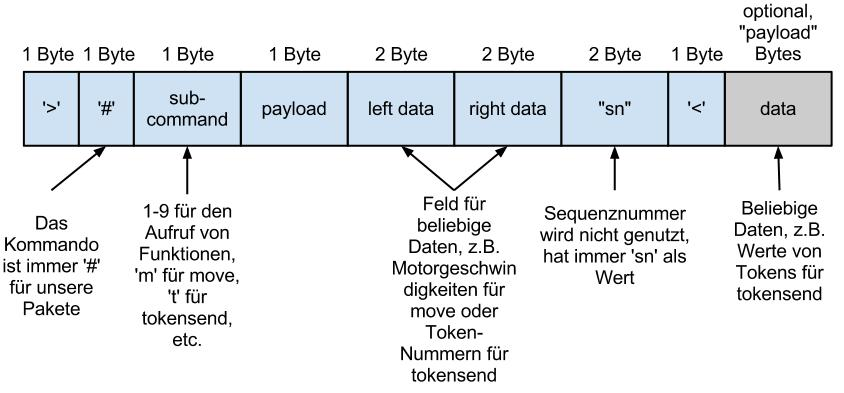
\includegraphics[scale=0.5]{pic/ctBotWlanKonkret}
		\caption{Konkreter Aufbau eines \textit{commands} für unsere Anwendung}
		\label{ctBotWlanKonkret}
	\end{figure}
	
	Hierzu kann z.B. das Tool \textit{sendip} verwendet werden. Ein Beispiel hierzu:\\
	\textit{\$ perl -e 'print "'\textgreater\#\textbackslash x02\textbackslash x06\textbackslash x03\textbackslash x11\textbackslash
    x02\textbackslash x02xy\textless hallo\textbackslash x00"'' \textgreater test.bin\\
    \$ sudo sendip -p ipv4 -is 192.168.0.234 -p udp -us 2000 -ud 10002 -f test.bin 192.168.0.9}\\
    Hierzu wird zunächst mit einem PERL print-Befehl ein Paket erzeugt und in eine Datei geschrieben und anschließen wird der Dateiinhalt mit \textit{sendip} an den Bot (hier 192.168.0.9) gesendet.
	(Die Paramter von links nach rechts: Protokoll IPv4, Quell-IP 192.168.0.234, Protokoll UDP, UDP-Quellport 2000, UDP-Zielport 10002, Datei (deren Inhalt gesendet werden soll) test.bin, die Ziel-IP 192.168.0.9)
	Der Grund für den Umweg über die Datei ist lediglich, dass man sich dadurch "'verlorene"' Zeichen oder kaputte Eingaben erspart, was der Fall wäre wenn man die Eingabe piped oder über eine Subshell erzeugt.
\end{itemize}
Die wesentlich einfachere Variante Pakete an den Bot zu schicken ist das Skript \verb+ctremote.py+ bzw. dessen Funktion \verb+send_cmd(...)+. Dazu siehe \ref{ctremote}.

\subsection{Zusatzaufgabe}

\subsubsection{ctremote.py - Ein Skript zur Fernsteuerung des Bots}
\label{ctremote}
Das Skript ist ein interaktives Programm, welches dem Nutzer ermöglicht Befehle einzugeben, die Aktionen auf Seiten des Bots auslösen. Dazu muss auf dem Bot das Programm laufen, welches in Abschnitt \ref{ctremote_bot} beschrieben ist.\\
Sieht der Nutzer folgenden Prompt, kann er Befehle eingeben:

\textbf{ctBot-remote \$}\\
Nachfolgend die bisher implementierten Befehle:
\begin{itemize}
	\item subcmd <subcommand>\\
	Sendet den angegebenen Subcommand <subcommand> an den Bot. Es sind bisher folgende Subcommands implementiert:
	\begin{itemize}
		\item 1 oder stand\\
		Lässt den Bot anhalten.
   		\item 2 oder motte1\\
   		Lässt den Bot die erste Implementierung von "'Motte"' ausführen.
   		\item 3 oder kakerlake1\\
   		Lässt den Bot die erste Implementierung von "'Kakerlake"' ausführen.
   		\item 4 oder motte2\\
   		Lässt den Bot die zweite Implementierung von "'Motte"' ausführen.
   		\item 5 oder kakerlake2\\
   		Lässt den Bot die zweite Implementierung von "'Kakerlake"' ausführen.
   		\item 6 oder acht\\
   		Lässt den Bot eine Acht fahren.
   		\item 7 oder linie\\
   		Lässt den Bot eine Linie entlang fahren.
	\end{itemize}
	Beispiel: \textit{subcmd motte1}
	
	Beispiel 2 : \textit{subcmd 6}
	\item move\\
	Nach Eingabe dieses Befehls ist der Bot über die Tastatur fernsteuerbar. Die Tastenbelegung dafür ist wie folgt:
	\begin{itemize}
		\item \textbf{W} Vorwärts fahren.
		\item \textbf{S} Rückwärts fahren.
		\item \textbf{A} Nach links drehen.
		\item \textbf{D} Nach rechts drehen.
		\item \textbf{E} Anhalten.
		\item \textbf{Q} Beendet den move-Befehl und kehrt zur Befehlseingabe zurück.
	\end{itemize}
	\item get <what>\\
	Zeigt einem den aktuellen Wert von <what> an. Dabei kann <what> momentan \textit{botip} (also die IP des zu steuernden Bots) oder \textit{port} (also der UDP-Port, über den kommuniziert wird) sein.
	
	Beispiel: \textit{get botip}
	\item set <what> <value>\\
	Setzt den Wert von <what> auf <value>. Hierbei kann <what> wieder \textit{botip} oder \textit{port} sein.
	
	Beispiel: \textit{set botip 192.168.0.9}
	\item help\\
	Gibt einen kurze Übersicht aller Befehle mit einer kurzen Beschreibung aus.
	\item help <cmd>\\
	Gibt einen detaillierten Hilfetext zum angegebenen Befehl <cmd> aus.
	
	Beispiel: \textit{help subcmd}
	\item exit\\
	Beendet das Skript.
	\item quit\\
	Beendet das Skript.
\end{itemize}
Die Tastenkombination \textit{STRG+C} wird von dem Skript abgefangen und sendet dem Bot sofort den Befehl zum Anhalten, beendet das Skript jedoch nicht. Um das Skript zu beenden muss einer der oben beschrieben Befehle \textit{quit} oder \textit{exit} verwendet werden.

\subsubsection{Aufbau von ctremote.py}
Das Skript besteht intern aus folgenden Funktionen:

\begin{itemize}
	\item \verb+help(cmd="")+\\
	Die Funktion bekommt einen optionalen Parameter \textit{cmd}. Wird kein Parameter übergeben, gibt die Funktion einen allgemeinen Hilfetext aus. Wird jedoch ein Befehl als Parameter übergeben, gibt die Funktion eine, für den übergebenen Befehl, passende Hilfe aus.
	\item \verb+openSocket()+\\
	Die Funktion öffnet einen neuen UDP-Socket mit IP und Port der aktuellen Konfiguration. (IP und Port entweder wie im Skript selbst hinterlegt oder mit dem \textit{set}-Befehl (siehe \ref{ctremote}) gesetzt.)
	\item \verb+send_cmd(subcmd,ldata="ld",rdata="rd",payload="\x00",data="")+\\
	Diese Funktion ist dafür zuständig ein Paket nach Norm des Bots (siehe \ref{wlan_auf_bot}) zusammenzubauen und schließlich an ihn zu senden.
	Der einzig zwingend nötige Parameter ist der Subcommand \textit{subcmd} (1 Byte), welcher dem Bot die auszuführende Aktion mitteilt.
	Optionale Parameter sind \textit{ldata} (2Byte) und \textit{rdata} (2 Byte), welche z.B. als Parameter für den Subcommand genutzt werden können, sowie \textit{payload} (1 Byte, Größe von \textit{data}) und \textit{data} (bis zu 255 Byte), welche genutzt werden können, wenn man zusätzliche Daten an den Bot senden will.
	Die Größe der Parameter ist dabei genau einzuhalten.
	\item \verb+recv()+\\
	Diese Funktion läuft während der gesamten Ausführung des Skripts als Thread und ist dafür zuständig Daten vom Bot zu empfangen und zu verarbeiten.
	\item \verb+user_input_eval(usrin)+\\
	Diese Funktion ist dafür zuständig die Eingaben des Nutzers zu interpretieren und die entsprechenden Aktionen durchzuführen, indem sie die anderen Funktionen des Skripts aufruft.
	Der zwingend anzugebende Paramter \textit{usrin} ist dabei die Eingabe des Nutzers.
	\item \verb+move()+
	In dieser Funktion läuft eine Schleife, welche dauerhaft die Tastatureingaben einliest und entsprechend der Eingabe den Bot fahren lässt (wozu sie intern \verb+send_cmd+ nutzt). Die Schleife wird erst duch drücken der Taste Q beendet.
\end{itemize}


\subsubsection{Programm auf dem Bot}
\label{ctremote_bot}
TODO: wie sieht das programm aus, welches die WLAN-pakete auswertet und aktionen auslöst blablabla...

